% !TEX root = paper.tex
\section{Trip Identification}\label{s.trips}

Let the $i_{th}$ sighting of vehicle \emph{k} be defined as the unordered pair:

\begin{equation} \label{e.sighting}
s^{k}_{i} = \{ c, t \}
\end{equation}

where \emph{c} is an integer that uniquely identifies a camera, and \emph{t} is a scalar representing a point in time (e.g.\ a timestamp).

Let an ordered sequence of sightings of vehicle \emph{k} define the $u_{th}$ trip of \emph{k}:

\begin{equation} \label{e.trip}
w^{k}_{u} = \left(s^{k}_{(1)}, s^{k}_{(2)}, \dots , s^{k}_{(n)}\right)
\end{equation}

where \( n \) is the length of the trip, i.e.\ the number of sightings. Moreover, let the corresponding journey time sequence, of length \(n-1\), be defined as the time difference of consecutive sightings:

\begin{equation} \label{e.journeytime}
jt^{k}_{u} = \left(t^{k}_{(2)} - t^{k}_{(1)}, \ldots, t^{k}_{(n)} - t^{k}_{(n-1)} \right)
\end{equation}

We consider a trip of \emph{k} valid if the following conditions are met:

\begin{align}
n &\ge 1 , \label{e.trip.constraints.1} \\
\tau_{(i)} &< jt^{k}_{u(i)} < \Tau_{(i)} \ , \ \forall i \in jt^{k}_{u(i)} \label{e.trip.constraints.2}
\end{align}

The first condition~\ref{e.trip.constraints.1} is straightforward and specifies that every trip should have at least one sighting. The second condition~\ref{e.trip.constraints.2} defines a minimum and maximum travel times between consecutive observations. Its purpose is twofold:
\begin{enumerate*}[label=(\roman*)]
  \item first, to allow trips made by the same vehicle to be differentiated. For instance, given two consecutive sightings of \emph{k} three hours apart, we want to interpret them as belonging to different trips of \emph{k};
  \item second, it allows unplausible trips to be identified. For example, an unplausible trip can result from observing \emph{k} at a given camera and then a few seconds later at a second camera, several miles apart. Two explanations are common, either one of the cameras made a detection error, or there is another vehicle with a cloned plate number travelling in the road network.
\end{enumerate*} Evidently, condition~\ref{e.trip.constraints.2} is only valid for trips of length two or greater. Nevertheless, trips can easily be differentiated by first sorting sightings by time of occurrence, then calculating the journey time sequence for the entire sequence and finally comparing each element against $\Tau$. An example of a trip identified this way can be seen in Figure~\ref{fig:trip-example}.

\begin{figure}[t]
  \centering
  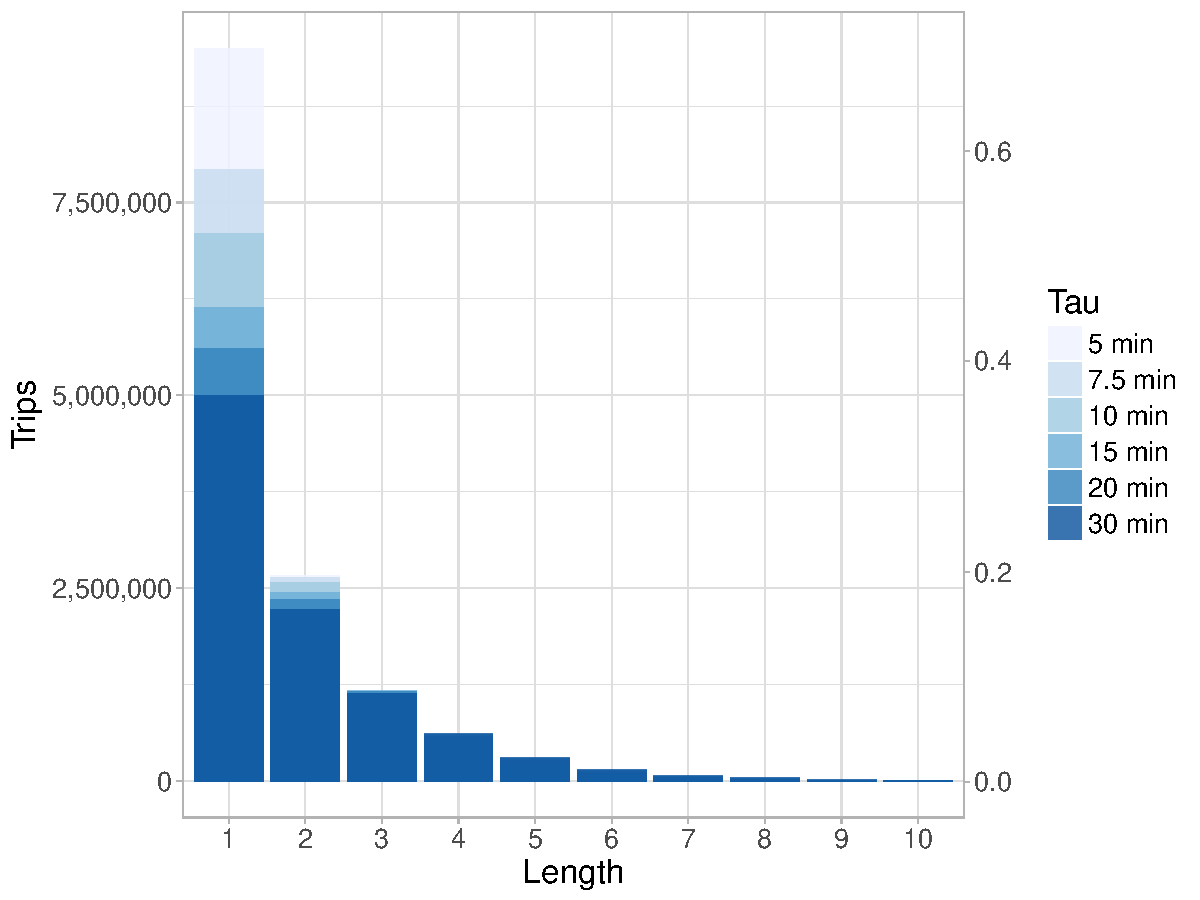
\includegraphics[width=1\linewidth]{length-dist.pdf}
  \caption{Distribution of trips per length of trip.}
  \label{fig:length-dist}
\end{figure}

\begin{figure*}[!ht]%
  \centering
  \begin{subfigure}[c]{.5\textwidth}
    \small
    \tabcolsep=0.09cm
    \begin{tabular}{c c c c c c c}
      \hline
      Vehicle & Camera & Timestamp & Trip & Sighting & \thead{Journey \\Time} & \thead{Trip \\Id}\\
      \hline
      2362920 & 1014 & \makecell{2017-02-01 \\ 00:00:06} &   1 &   1 & NA & 21 \\
      2362920 & 1044 & \makecell{2017-02-01 \\ 00:01:28} &   1 &   2 & 82.38 & 21 \\
      2362920 &  35 & \makecell{2017-02-01 \\ 00:02:32} &   1 &   3 & 63.50 & 21\\
      2362920 &  32 & \makecell{2017-02-01 \\ 00:04:38} &   1 &   4 & 125.95 & 21\\
       \hline
    \end{tabular}
    \label{fig:trip-example-table}
  \end{subfigure}\hfill
  %\qquad
  \begin{subfigure}[c]{.48\textwidth}
    \centering
    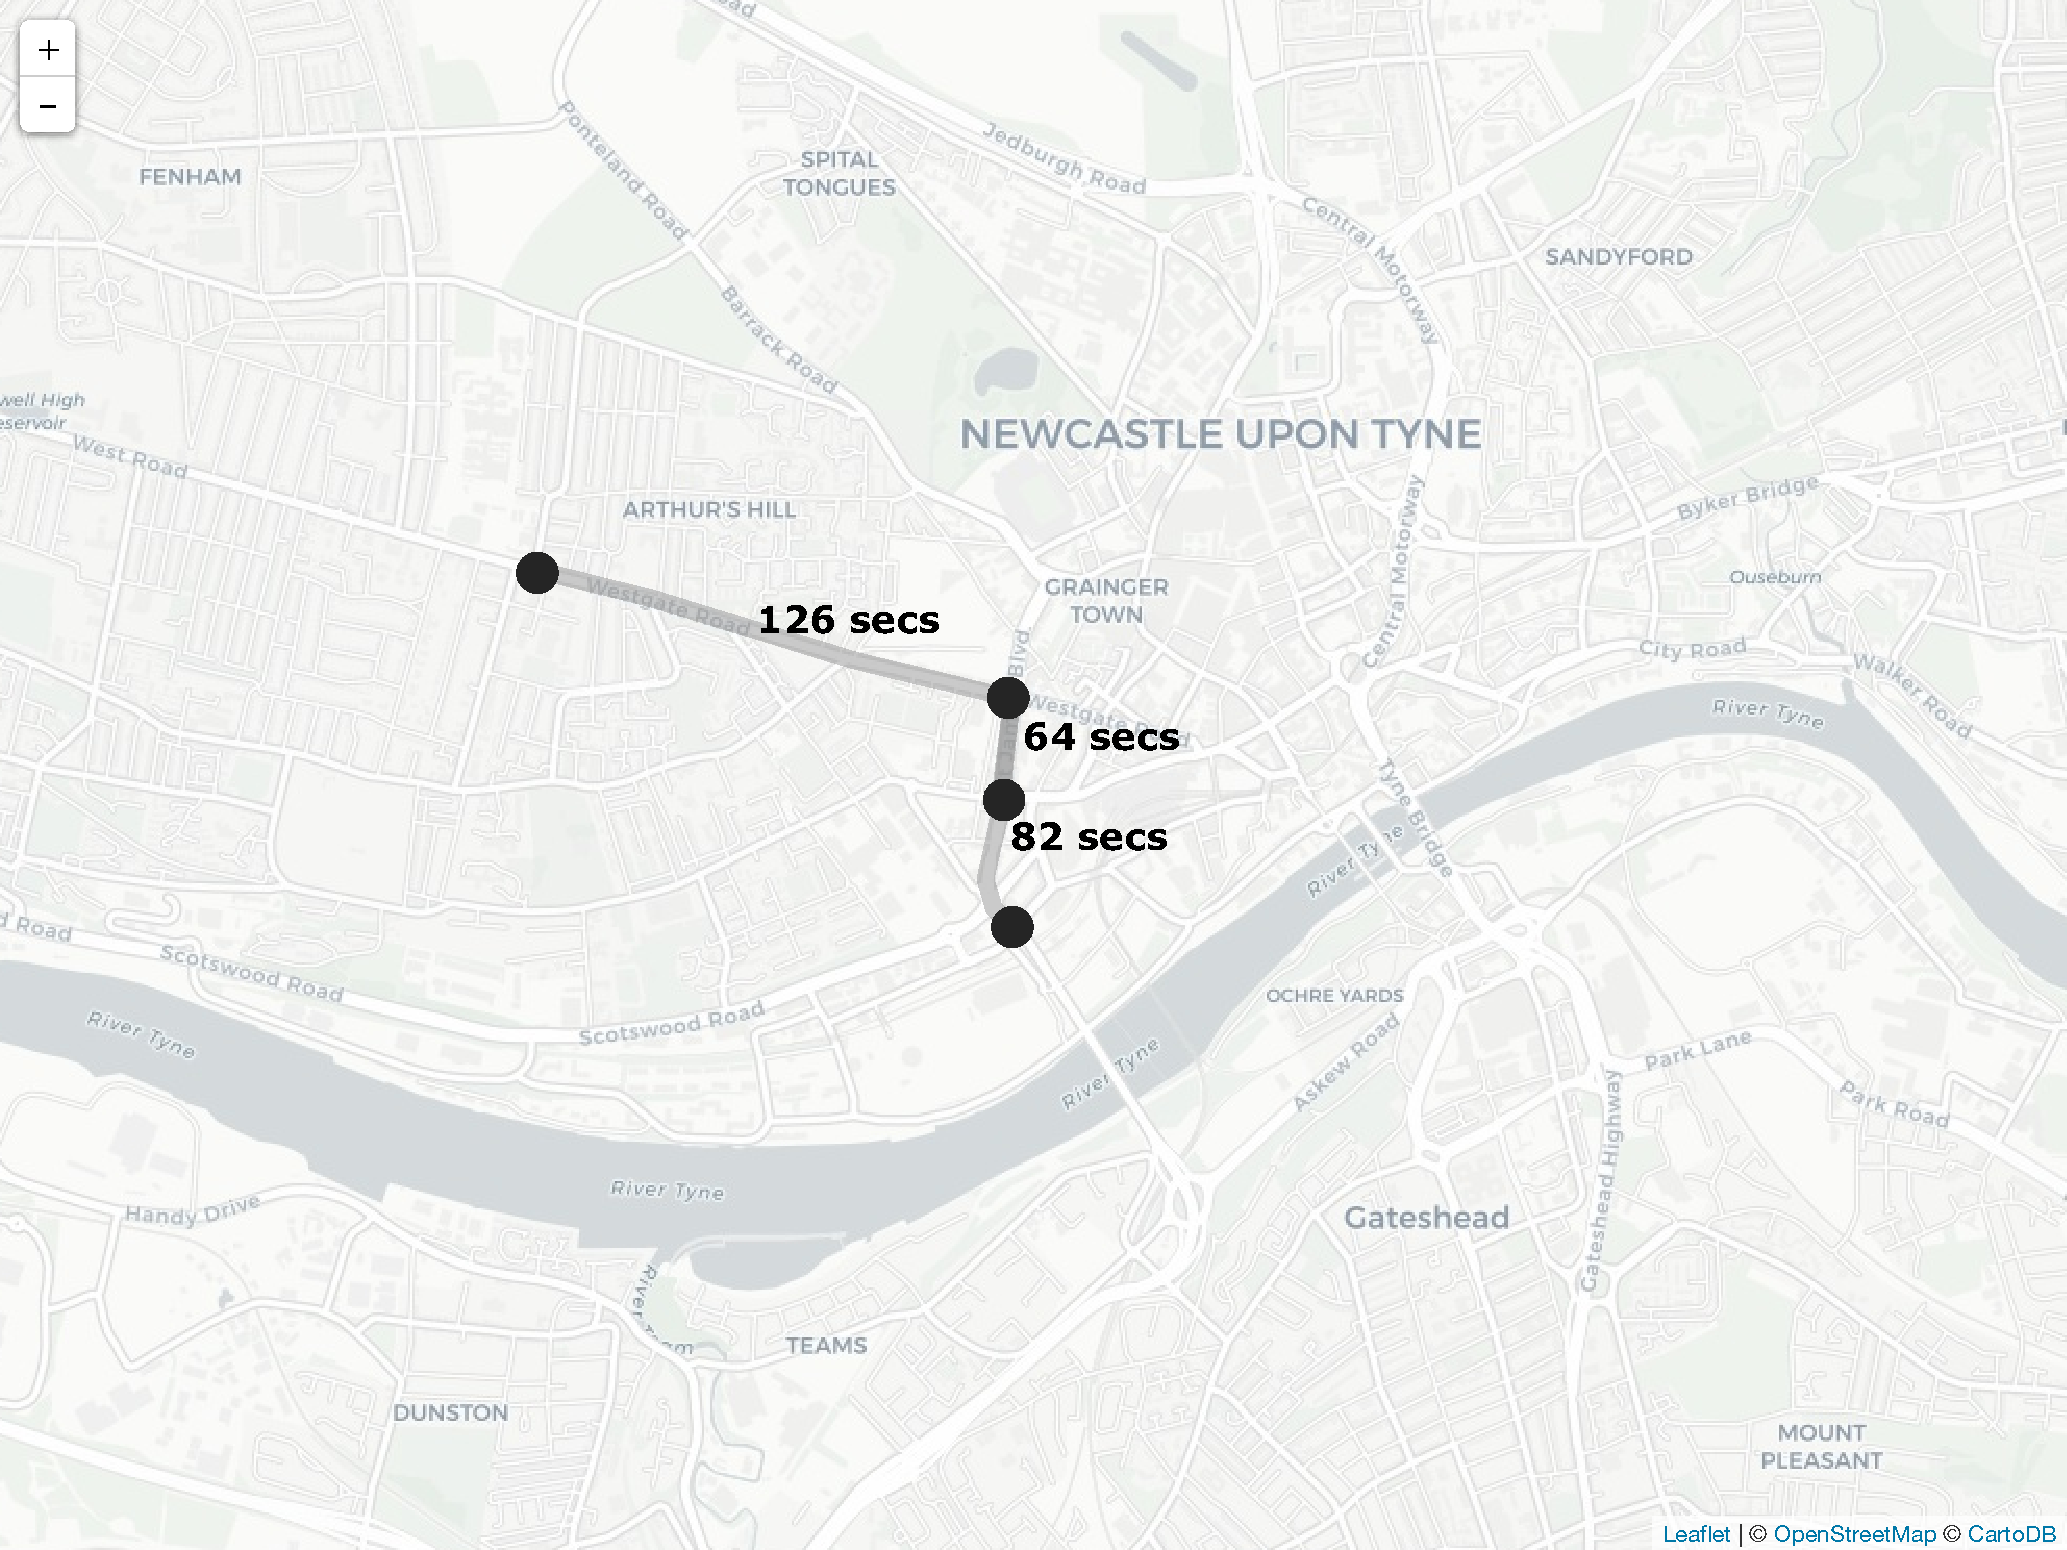
\includegraphics[width=1\linewidth]{trip-example.pdf}
    \label{fig:trip-example-map}
  \end{subfigure}\hfill
  \caption{Example of a trip of length 4. On the left side the correspoding data table is shown. The $u_{th}$ trip of each vehicle is given by the variable \emph{Trip}, whereas the $i_{th}$ sighting is given by variable \emph{Sighting}. The variable \emph{JourneyTime} gives the travel time from the previous to current sighting. Lastly, the variable \emph{TripId} represents the unique sequence of cameras that describes the trip. This allows trips to be grouped and summarised not only in terms of their origins and destination, but also routes. On the right side, the same trip is plotted on a map. However, the lines do not represent the true route taken by the vehicle, but instead the fastest driving route between sightings. Even though no routing information is available for each consecutive pair of sightings, the observed journey times can be compared against the distribution of collective journey times to rank the set of most likely routes chosen (which can be determined for instance by Stochastic User Equilibrium~\cite{Castillo2008}).}%
  \label{fig:trip-example}%
\end{figure*}

The simplest approaching to choosing the value of $\Tau$ is to pick a fixed empirical value, such as 5 or 10 minutes. However, if the distance between two cameras is greater than another origin-destination (od) pair of cameras, then it makes sense that $\Tau$ is relaxed. Similarly, if there is an anomaly in the road network, such as a traffic jam, and the routes connecting the two cameras are affected, then the value of $\Tau$ should also be adapted. Hence, $\Tau$ should be a function of the distance between the two cameras (or, more accurately, of the top n-routes between these) and the distribution of observed journey times. The same rationale can be applied to estimating $\tau$.

On the other hand, a consistent set of models and methodologies for estimating $\Tau$ and $\tau$, under a variety of circumstances and road anomalies, remains an open research problem. Thus, for the purposes of this work, we will consider these parameters to be fixed. Nevertheless, the importance of estimating these parameters should not be understated. Any errors in trip identification that occur due to poor estimation and filtering methods will propagate and be amplified in posterior analysis done using trip data. Therefore, $\Tau$ and $\tau$ estimation is something that needs to be carefully addressed and studied in the future in order to fully understand its impact in the outcome of the research. To briefly exemplify this, figure~\ref{fig:length-dist} shows how the number of trips per length of trip varies by fixing $\Tau$ at different empirical values ($\tau$ is ignored).

\subsection{Duplicate scannings}

To ensure that every trip of vehicle \emph{k} is unique in the sequence of all valid trips of vehicle \emph{k}:

\begin{align}
W^{k} = \left( w^{k}_{(1)}, w^{k}_{(2)}, \ldots, w^{k}_{(N)} \right) \label{e.trip.history}
\end{align}

where \emph{N} is the number of trips of \emph{k}, then there should be no two trips containing the same sighting:

\begin{align}
s^{k}_{(u(i))} \neq s^{k}_{(v(j))}, \forall u,v &= 1, 2, \ldots, N \ , \ u \neq v,  \label{e.trip.history.constraint} \\
\forall i,j &= 1, 2, \ldots, n \ , \ i \neq j \nonumber
\end{align}

However, ANPR can identify the same vehicle multiple times in the same run, if for instance the vehicle is stopped at a junction or traffic light. Hence, if two sightings occurred at the same location in a very short period of time, then there is a strong possibility that these are duplicate observations. As a simplification, we can assume that a trip should not contain cycles and that no camera should appear twice in the same trip. Yet, this assumption ignores cases where a vehicle is required to correct its route by passing through the same location as one previously observed in the same trip. Thus, we affirm that two sightings of vehicle \emph{k} are different if they were observed at two different points in time at different locations, or, if observed at the same location, then the time interval must be greater than a parameter $\gamma$, otherwise the two sightings are deemed as duplicates:


\begin{align} \label{e.sighting.different.2}
 (\ c^{k}_{i} &\ne c^{k}_{j} \, )\ \vee \\
 (\ c^{k}_{i} &= c^{k}_{j} \wedge |t^{k}_{i} - t^{k}_{j}| < \gamma \, )\ \Rightarrow s^{k}_{i} \ne s^{k}_{j}  \ , \ i \ne j \nonumber
\end{align}

 Although the estimation of $\gamma$ carries similar considerations and consequences as those of estimating $\Tau$ and $\tau$, most duplicates can be identified in consecutive sightings of the same camera within the same trip. Even though a poor estimation of $\gamma$ also has impact in error propogation, this decreases substantially after filtering duplicates according to the heuristic above, due to the low occurrence of cycles in trips. Nevertheless, this issue needs to be fully investigated in future works.

\subsection{Errors in plate scanning}

Number plate recognition cameras have accuracy rates of 99.9\% or higher. If we consider that on average 1 to 10 out of 10000 scans are misclassified plate number then approximately 200 to 2000 scans everyday are incorrect scans. We categorise the errors made by ANPR cameras into two types:
\begin{enumerate}
  \item a passing vehicle is not detected by the camera;
  \item a different vehicle is detected instead.
\end{enumerate}
In the first case, there is no observed data. The corresponding trip sequence for the affected vehicle will be missing a sighting but we will have no indication of this. On the second case, there is a recorded sighting, but this will be assigned to the incorrect vehicle. Even though, the camera provides a value of \emph{confidence} which helps in diagnosing incorrect scans, errors still occur for high values of confidence. Even though that in this work we do not present a complex solution for this issue, methods to detect and address these two types of errors need to be designed and implemented in the future.
